\documentclass[review]{elsarticle}
\journal{Information Systems}

\newtheorem{obs}{Observation}[section]
\newtheorem{theorem}{Theorem}
\newtheorem{coro}{Corollary}
\newcommand{\bss}{\mathcal{S}}
\newcommand{\C}{\mathcal{C}}
\newcommand{\D}{\mathcal{D}}
\newcommand{\svs}{\textit{svs}}
\newcommand{\bys}{\textit{bys}}
\newcommand{\merge}{\textit{merge}}
\newcommand{\seq}{\textit{seq}}
\newcommand{\bs}{\textit{bin}}
\newcommand{\expon}{\textit{exp}}
\newcommand{\lookup}{\textit{lookup}}
\newcommand{\repair}{Re-Pair}
\newcommand{\lzend}{LZ-End}
\newcommand{\lzma}{LZMA}

\newcommand{\uilib}{{\tt uiHRDC}}

\newcommand{\vbyte}{\texttt{Vbyte}}
\newcommand{\vbyteB}{\texttt{VbyteB}}
\newcommand{\rice}{\texttt{Rice}}
\newcommand{\riceB}{\texttt{RiceB}}
\newcommand{\simplen}{\texttt{Simple9}}
\newcommand{\simpled}{\texttt{Simple16}}
\newcommand{\pfordelta}{\texttt{PforDelta}}
\newcommand{\qmx}{\texttt{QMX}}
\newcommand{\riceRuns}{\texttt{Rice-Runs}}
\newcommand{\simpleRuns}{\texttt{Simple9-Runs}}
\newcommand{\pfordeltaRuns}{\texttt{PforDelta-Runs}}
\newcommand{\vbyteCM}{\texttt{Vbyte-CM}}
\newcommand{\vbyteCMB}{\texttt{Vbyte-CMB}}
\newcommand{\vbyteST}{\texttt{Vbyte-ST}}
\newcommand{\vbyteSTB}{\texttt{Vbyte-STB}}
\newcommand{\repairNo}{\texttt{RePair}}
\newcommand{\repairSkip}{\texttt{RePair-Skip}}
\newcommand{\repairSkipCM}{\texttt{RePair-Skip-CM}}
\newcommand{\repairSkipST}{\texttt{RePair-Skip-ST}}
\newcommand{\vbyteLZMA}{\texttt{Vbyte-LZMA}}
\newcommand{\vbyteLzend}{\texttt{Vbyte-Lzend}}
\newcommand{\rlcsa}{\texttt{RLCSA}}
\newcommand{\wcsa}{\texttt{WCSA}}
\newcommand{\slp}{\texttt{SLP}}
\newcommand{\wslp}{\texttt{WSLP}}
\newcommand{\lzindex}{\texttt{LZ77-index}}
\newcommand{\lzendindex}{\texttt{LZend-index}}

\newcommand{\interpolative}{\texttt{Interpolative}}
\newcommand{\efopt}{\texttt{EF-opt}}
\newcommand{\optpfd}{\texttt{OPT-PFD}}
\newcommand{\varint}{\texttt{varintG8IU}}

\usepackage{fullpage}
\usepackage{comment}
\usepackage{url}
\usepackage{colortbl}
\usepackage[usenames]{xcolor}

\newcommand{\highlight}[1]{\textcolor{red}{#1}}



\begin{document} 
\begin{frontmatter}	
	\title{Report from Docker Container\\ Reproducing Experiments from paper: Universal Indexes for Highly Repetitive Document Collections\tnoteref{t1}, by:}
	\tnotetext[t1]{}


	\author[udc]{Antonio Fari\~na\corref{cor1}}
	\ead{fari@udc.es}

	\author[uva]{Miguel A. Mart\'inez-Prieto}
	\ead{migumar2@infor.uva.es}

	\author[udp]{Francisco Claude}
	\ead{fclaude@recoded.cl}

	\author[uchile]{Gonzalo Navarro}
	\ead{gnavarro@dcc.uchile.cl}
	
	\author[ny]{Fernando Chirigati}
	\ead{fchirigati@nyu.edu}

	\cortext[cor1]{Corresponding author}	

	\address[udp]{Escuela de Inform\'atica y Telecomunicaciones, Universidad Diego Portales, Chile.\\}
	\address[udc]{Database Laboratory, University of A Coru\~na, Spain.\\}
	\address[uva]{DataWeb Research, Department of Computer Science, University of Valladolid, Spain.}		
	\address[uchile]{Department of Computer Science, University of Chile, Chile.}

	\address[ny] {Department of Computer Science and Engineering, New York University, New York City, NY, United States.}

	\begin{abstract}
We include in this report the main figures reproduced for paper \cite{CFMNis16.3} from the experimental data and source codes obtained by
running our build, search, and report scripts from our original paper, and described in detail in our reproducibility paper: {``\em Reproducible Research about Indexing Repetitive Document Collections''}.
\bigskip
\noindent

{\bf Keywords:} {\em experiments, reproducibility.}
	\end{abstract}

\end{frontmatter}



%%%%%%%%%%%%%%%%%%%%%%%%%%%%%%%%%%%%%%%%%%%%%%%%%%%%%%%%%%%%%%%%%%%%%%%%%%%%%%%%%%%%%%%%% 
%%%%%%%%%%%%%%%%%%%%%%%%%%%%%%%%%%%%%%%%%%%%%%%%%%%%%%%%%%%%%%%%%%%%%%%%%%%%%%%%%%%%%%%%% 
\section{Experimental Framework and Results}

We experimentally study the space/time tradeoffs obtained with the described 
inverted list representations, in both the non-positional and positional 
scenarios. In the positional scenario we also add a comparison with the 
self-indexes proposed.

\subsection{Test Data} \label{sec:testdata}
Within \uilib\ we provide in \texttt{data} directory, both the document collections and the query sets used in the experimental setup of our original paper.
They are described below.

\subsubsection{Document Collections}

Our document collections were created from the 108.5 GB Wikipedia collection described by He et al.~\cite{HZS10}, which contained 10\% of 
the complete English Wikipedia from 2001 to mid 2008. It contains 240,179 articles, and each of them has a number of versions. Its statistics
are shown in Table~\ref{tab:coll}. Note that we had not the original 108.5 GB collection, but a filtered (tag-free) version of it whose size
totaled 85.58 GB. Therefore, the original collection was $1.27$ times larger than ours.

\begin{table*}[htb]
	{\small
		\begin{center}
			\begin{tabular}{|l|r|r|r|r||r|r|}
				\hline                                                                                           
				Subset   & Size~~ & Articles & Number of & Versions / &       {Filename}         &        {Filesize}  \\
				         & (GB)~  &          & versions  & article~~~ &     (within \uilib)      &        {(GB)}      \\
				\hline                                                                                           
				\hline                                                                                           
				Full     & 108.50 &  240,179 & 8,467,927 &      35.26 &        {\tt --}          &            {85.58} \\
				Non-pos  &  24.77 &    2,203 &   881,802 &     400.27 &        {text20gb.txt}    &            {19.53} \\
				Pos      &   1.94 &    4,327 &   149,761 &      34.61 &       { wiki\_src2gb.txt}&             {1.94} \\
				\hline                                                                                           
				
			\end{tabular}
		\end{center}
	}
	\caption{Detailed statistics of the document collections used.} 
	\label{tab:coll}
\end{table*}

From the {\tt Full} collection of articles, we chose two subsets of the articles, and collected all the versions of the chosen articles. 
For the non-positional setting our subset (\texttt{Non-pos}) contains a prefix of 19.53 GB of the full collection, whereas for positional indexes we
chose 1.94 GB of random articles. However, for a fair comparison with the techniques from~\cite{HZS10}, in the non-positional scenario we scaled the size
of the \texttt{Non-pos} subset using the above $1.27$ factor when referring to its space requirements. Additional statistics of our two subsets are
also included in Table~\ref{tab:coll}.

%
%Table~\ref{tab:coll} also provides the statistics of our two subsets. As it can be 
%seen, the 24.77 GB prefix is more repetitive than the full collection, whereas
%the 1.94 GB subcollection is similar to the global collection.


\subsubsection{Query sets}

Since the experiments target at providing space/time for the different indexing alternatives 
when performing \texttt{locate(pattern)} and \texttt{extract(interval)} queries we provided two types
of query sets for each document subcollection.

\begin{itemize} 
	\item Query sets for \texttt{locate}: We provide four query sets, each of them containing 1,000 queries, which include:
	{\em i)} two query sets composed of one-word patterns chosen at random from the vocabulary of the indexed subcollection. In the first
	case ({\em W$_a$}), it includes low-frequency words occurring less than 1,000 times. In the second case, the query set ({\em W$_b$}) includes
	high-frequency words occurring more than 1,000 times; {\em and ii)} two query sets with 1,000 phrases composed of 2 and 5 words that
	were chosen randomly from the text of the subcollection (with no restrictions on its frequency).
	
	\item Interval sets for \texttt{extract}: Aiming at measuring extraction time when recovering snippets of length 80 (around one line) and 13,000 (around one document, in our
	collection) characters, we generated: {\em i)} a set of 10,000 intervals of width 13,000 characters from the {\tt POS} text collection, and {\em ii)}  a set containing
	100,000 intervals of width 80 characters. Since these intervals are not suitable for our word-based self-indexes (\wcsa\ and \wslp), and assuming that the average word length 
	is around $4$ in our datasets, we also generated two additional sets composed respectively of 10,000 intervals containing $3,000$ words each, and	
	and 100,000 intervals containing $80$ words each.
\end{itemize}



\section{Techniques used: Inverted indexes and self-indexes}
The techniques included  in this Report are summarized in Table~\ref{tab:techniques}. Recall that we include, compressed inverted indexes for the non-positional scenario, whereas for the positional scenario we include the most promising compressed inverted indexes and also self-indexes.

\begin{table}[htbp]
	\caption{Techniques included in this report.}
	\begin{center}
	
	\scriptsize
	\begin{tabular}{|l|l|l|}
	\hline
	\textbf{NON POSITIONAL INV. INDEXES} & \textbf{POSITIONAL INV. INDEXES} & \textbf{SELF-INDEXES} \\ \hline
	\hline
	\hline
	RICE                      &  RICE                    & WCSA \\ \hline
	RICE-B              &                          & RLCSA \\ \hline
	VBYTE                     &  VBYTE                   & SLP \\ \hline
	VBYTE-CM                  &  VBYTE-CM                & WSLP \\ \hline
	VBYTE-ST                  &  VBYTE-ST                & LZ77-Index \\ \hline
	VBYTE-B              &                          & LZEnd-Index \\ \hline
	VBYTE-CM-B           &                          & \multicolumn{1}{c|}{} \\ \hline
	VBYTE-ST-B &                          &  \\ \hline
	SIMPLE-9                  &  SIMPLE-9e                &  \\ \hline
	PFORDELTA                 &                          &  \\ \hline
	QMX-SIMD                  &  QMX-SIMD                &  \\ \hline
	*ELIAS-FANO-OPT           &  *ELIAS-FANO-OPT         &  \\ \hline
	*OPT-PFD                  &  *OPT-PFD                &  \\ \hline
	*INTERPOLATIVE            &  *INTERPOLATIVE          &  \\ \hline
	*VARINT-G8IU              &  *VARINT-G8IU            &  \\ \hline
	RICE-RLE                  &                          &  \\ \hline
	VBYTE-LZMA                &  VBYTE-LZMA              &  \\ \hline
	VBYTE-LZEND               &                          &  \\ \hline
	REPAIR                    &  REPAIR                  &  \\ \hline
	REPAIR-SKIPPING           &  REPAIR-SKIPPING         &  \\ \hline
	REPAIR-SKIPPING-CM        &  REPAIR-SKIPPING-CM      &  \\ \hline
	REPAIR-SKIPPING-ST        &  REPAIR-SKIPPING-ST      &  \\ \hline
	\hline
	\textit{(text not included, only intersections)} & \textit{(text compressed with Re-pair)} &  \\ 
		\hline
	\end{tabular}
	\label{tab:techniques}
	\end{center}
\end{table}





%%%%%%%%%%%%%%%%%%%%%%%%%%%%%%%%%%%%%%%%%%%%%%%%%%%%%%%%%%%%%%%%%%%%%%%%%%%%%%%%
\subsection{Results for Non-positional inverted indexes}

Our experiments compare the space/time tradeoffs of several variants of 
non-positional inverted indexes over the highly repetitive 24.77 GB subcollection described above. We include in this comparison some of the best classical encodings to represent d-gaps, such as \rice, \simplen, 
\pfordelta, and \vbyte\ with no sampling to speed up intersections (thus only merge-wise intersections are feasible). 
 %
We also include two alternatives using \vbyte\ coupled with list sampling \cite{CM10} (\vbyteCM) with $k=\{4,32\}$, or domain sampling \cite{TS10} (\vbyteST) with $B=\{16,128\}$. In addition, we include the hybrid variant of \vbyteCM\ that uses bitmaps to represent the largest inverted lists (\vbyteCMB) \cite{CM10}. For completeness we used the same approach on \vbyteST, to build \vbyteSTB, and also included variants \vbyteB\ and \riceB\ with no sampling.
 %
We also tested the novel \qmx\footnote{\url{http://www.cs.otago.ac.nz/homepages/andrew/papers/QMX.zip}. } technique \cite{trotman2014} that uses SIMD-instructions to boost decoding of large lists, and coupled it with an intersection algorithm \cite{Lemire2015:simdInt} that also benefits from SIMD-instructions.\footnote{ \url{https://github.com/lemire/SIMDCompressionAndIntersection}. In this case we had to use \texttt{g++} version 4.7 with the \texttt{-O3 -msse4} flags, according to authors' sources.}
 %
 %/usr/bin/g++-4.7 -O3 -msse4 -mavx -std=c++11  -Weffc++  -ggdb -DDEBUG=1 -D_GLIBCXX_DEBUG 
 % gcc version 4.7.3

We also tested the recent Partitioned Elias-Fano indexes \cite{OV14}, and used the best/optimized variant from that paper (\efopt). The source code is available at authors' website.\footnote{\url{https://github.com/ot/partitioned_elias_fano.}}
From  the same authors \cite{OV14}, we also included in our experiments the variants \optpfd\ (optimized PForDelta variant \cite{YDS09}), \interpolative\ (Binary Interpolative Coding \cite{MS00}), and \varint\ (SIMD-optimized Variable Byte code \cite{Stepanov:2011}). Since we used the implementations from \cite{OV14} and we adapted our query patterns to match their needs, or even measured partial times (parsing and map-to-documents) separately, we marked with an `\texttt{*}' these techniques in the figures. 

 %
 % CMAKE -DCMAKE_BUILD_TYPE=Release 
 % Options -msse4.2 -std=c++11
 % /usr/bin/g++-4.8 
 % gcc version 4.8.2


We compare all those techniques in Section~\ref{exp:nopos:others}, to determine which of the traditional techniques perform best in the repetitive scenario. 
Then, in Section~\ref{exp:nopos:ours} we compare them with the new variants designed to deal with repetitive data we proposed. In particular, we include \riceRuns,
\vbyteLZMA,  \vbyteLzend, \repairNo, \repairSkip. We add no sampling to them. Therefore, only \repairSkip\ can benefit of additional data to boost the intersections (which are performed sequentially). In addition, we show the \repair\ variants using sampling, \repairSkipCM\ (with $k=\{1,64\}$) and \repairSkipST\ (with $B=\{16, 256, 1024\}$). For \vbyteLzend\ we will obtain different space/time tradeoffs by tuning its {\em delta-codes-sampling} parameter $ds$ (see \cite{KNtcs12} for details) to $ds=\{4,16,64,256\}$.

Finally, note that the space results reported for the indexes are shown as a percentage 
of the index size with respect to the size of the original [sub]collection in plain text
($index\_size / original\_size \times 100$). Note that we are not considering in
this experiment the compressed representation of the text. 
Times are shown in microseconds per occurrence.



\subsubsection{Using traditional techniques in a repetitive scenario} \label{exp:nopos:others}

We include a comparison of well-known techniques that were initially developed
for non-repetitive scenarios, now operating on repetitive collections.
 % 
Figure \ref{fig:nonpos} shows the space/time tradeoffs for 
non-positional indexes using those techniques to represent posting lists. 

\begin{figure}[t]
\begin{center}
\includegraphics[angle=-90,width=0.49\textwidth]{../figures/f1/words1-1000/nonpos-Wa.eps}
\includegraphics[angle=-90,width=0.49\textwidth]{../figures/f1/words1001-100k/nonpos-Wb.eps}
\includegraphics[angle=-90,width=0.49\textwidth]{../figures/f1/phrases2-2/nopos-2_2.eps}
\includegraphics[angle=-90,width=0.49\textwidth]{../figures/f1/phrases5-5/nonpos-5_5.eps}
\caption{Space/time tradeoffs for non-positional indexes using traditional
techniques. Logscale.}
\label{fig:nonpos}
\end{center}
\end{figure}


%We can see that, among classical compression methods, both 
%\simplen\ and \pfordelta\ are much better in space than the older techniques like 
%\rice\ (one third of the space) and \vbyte\ (one fifth of the space). In typical 
%collections \rice\ achieves the best space, but these newer methods take 
%advantage of the many runs of 1s. They are also several times faster than
%\rice, and roughly as fast as \vbyte\ on word queries. On conjunctive queries, 
%however, \vbyte\ is faster. In those queries,
%adding samples to support \lookup-type intersections is advantageous: \vbyteST\ 
%is significantly faster than \vbyte\ (more than 3 times faster on 5-word
%queries). Surprisingly, in our experiments \vbyteCM\ (sampling to support \svs\ with exponential
%search on the longest list) turned out to be a bad choice, obtaining worse results than the simple
%\vbyte\ with no sampling. Note that the increase of time needed to recover an inverted list is due to 
%the fact that values stored in the samples are removed from the differential sequence, what adds an
%additional branch at decompression time.
%Using hybrid techniques (representing the longest inverted lists with bitmaps and \vbyte\ for the others) turned out to be a good choice, as both space and time are improved with respect to  the non-hybrid \vbyte\ variants. In the case of \rice, the \riceB\ hybrid counterpart did not improve space (as expected, since \rice\ is a bit-wise technique), yet the intersection times benefit significantly from the fast direct access to the longest lists.
%
%The novel \qmx\ shows to be an extremely fast technique when we deal with long posting lists (otherwise it cannot benefit from SIMD-optimized decompression) and the SIMD-based intersection algorithm \cite{Lemire2015:simdInt} outperforms the others for long conjunctive queries. Unfortunately, its space is high, even worse than \vbyte.
%
%The comparison with the Elias-Fano indexes \cite{OV14} shows that the recent \efopt\ performs very well in the repetitive scenario. It obtains the best overall space (half the space of the above \pfordelta\ variant). It also outperforms \interpolative\ in time, and is close to the times of \optpfd\ (which requires around 20\% more space). Technique \varint\ is the fastest of this group \cite{OV14}, yet as expected its space usage is far from the best ones (it is slightly worse than \vbyte). The conjunctive queries using these techniques are very fast. The use of a two-level structure enables an intersection algorithm (similar to {\em sequential}) where the candidate/eliminator from the shortest list is searched for in the others using {\em{next\_geq()}} built-in operator. Their implementation is however somehow slow on word queries, mainly because list elements are recovered one at a time by using an operator {\em next}. Note that \varint\ (the SIMD-optimized \vbyte) is slightly slower than our implementation of \vbyte\ even when fetching the posting lists of frequent words.
%
%%%%elige la más corta como candidato y las busca en las demás usando el operador next_geq
% 
%For the comparison with our new techniques, considering the scope of our
%article, we have retained three of those techniques, whose space usage is under 1\%: {\em i)} \simplen, which offers good performance both for word and 2-word conjunctive queries; {\em ii)} \efopt, which obtains the best space values and still good performance; and {\em iii)} \optpfd, which obtains space close to that of \efopt\ and slightly better performance both for word and conjunctive queries.

\subsubsection{Comparison with our proposals} \label{exp:nopos:ours}

Our next experiments compare our proposals with the best counterparts from the previous section. Figure \ref{fig:nonpos2} shows the space/time tradeoffs for all the resulting non-positional indexes. 

%The most important conclusion with regard to classical encoding methods is that they are unsuitable for highly repetitive collections.
%Our new techniques take one order of magnitude less space than \simplen\, and up to 5 times less space than \efopt. Yet, they are also significantly slower than the fastest classical variants. 

\begin{figure}[t]
\begin{center}
\includegraphics[angle=-90,width=0.49\textwidth]{../figures/f2/words1-1000/nonpos-Wa.eps}
\includegraphics[angle=-90,width=0.49\textwidth]{../figures/f2/words1001-100k/nonpos-Wb.eps}
\includegraphics[angle=-90,width=0.49\textwidth]{../figures/f2/phrases2-2/nopos-2_2.eps}
\includegraphics[angle=-90,width=0.49\textwidth]{../figures/f2/phrases5-5/nonpos-5_5.eps}
\caption{Space/time tradeoffs for non-positional indexes, comparing the best
classical techniques with our new ones. Logscale.}
\label{fig:nonpos2}
\end{center}
\end{figure}





%	Our first simple method to take advantage of repetitiveness, \riceRuns, makes
%	an interesting leap in space, from 1\% taken by \simplen\ or 0.5\% taken by \efopt, to
%	around 0.3\%. If we compare it in Figure~\ref{fig:nonpos} we can see that it takes one tenth the space of plain \rice\ and is at the same time faster, as it needs much less decompression work. It does 
%	not, however, get close to the space of stronger methods like \vbyteLZMA, which
%	achieves around 0.2\% space by exploiting other types of redundancy. However,
%	\riceRuns\ is significantly faster than \vbyteLZMA\ (up to 3 times).
%	
%	
%	
%	\vbyteLZMA\ is close to the smallest space that we can achieve. It is
%	significantly faster than \repairNo\ (up to 10 times) and than \repairSkip\ 
%	(up to 3 times) at word queries, as it decompresses faster the inverted list. 
%	However, on conjunctive queries, where many of the decoded values have to be 
%	discarded, the ability of \repairSkip\ to skip nonterminals without 
%	decompressing them finally makes it almost twice as fast as \vbyteLZMA,
%	and even faster than \riceRuns.
%	
%	As expected, \vbyteLzend\ succeeds at exploiting inter-list regularities 
%	and almost halves the space of \vbyteLZMA, yet it is by far the
%	slowest technique in our comparison, being more than an order of magnitude slower than \vbyteLZMA.
%	
%	Note that \repairNo\ obtains lower space (85\%) than \vbyteLZMA, despite the 
%	fact that LZ77 compression is more powerful than \repair. This is a
%	consequence of \lzma\ exploiting only intra-list regularities, and, as in \vbyteLZMA, shows that 
%	significant further repetitions are captured when considering the inter-list 
%	redundancies. The skipping information added to \repairNo\ adds very
%	little space (6\%), but significantly improves its time performance (almost 20
%	times faster on long phrases). This improvement occurs even on one-word queries
%	(up to 2.6 times faster), since \repairSkip\ does not need to carry out $rank$ 
%	operations on $R_B$ (recall Section~\ref{sec:repair}). Results also show that it is not
%	worth adding
%	sampling to \repairSkip. Sampling increases the space requirements, but no
%	improvements at intersections upon \repairSkip\ are reported by \repairSkipCM\ nor  \repairSkipST.
%	Note that for \repairSkipST\ we are showing only the plot corresponding to sampling 
%	parameter $B=1024$, which obtained the least space, since we obtain no time 
%	improvements and space usage grew from 25\% to 700\% using smaller values.






%%%%%%%%%%%%%%%%%%%%%%%%%%%%%%%%%%%%%%%%%%%%%%%%%%%%%%%%%%%%%%%%%%%%%%%%%%%%%%%%%%%%%%%%%%%%%%%%%%%%%%%%%%%%%
\subsection{Results for Positional indexes}

\begin{comment}
For testing the positional indexes we used the smaller subcollection, 
because several self-index implementations are unable to handle 
texts larger than 2 GB. 
q

For this scenario we used an Intel(R) Xeon(R) E5335 CPU running at 2.00 GHz, 
4 MB cache, 16 GB of RAM memory, 8 cores. 
The operating system installed is an Ubuntu GNU/Linux version 8.04.4 LTS 
running kernel 2.6.24-29-server (64 bits) and \verb|g++| compiler version 
4.2.4. Our code was compiled with the \verb|-O9| directive. We measure user 
times.
\end{comment}


For testing the positional indexes we used the 1.94 GB subcollection 
because several self-index implementations are unable to handle 
texts larger than $2^{31}$ bytes. 

Since self-indexes must reproduce the precise text, we cannot apply case
folding nor any kind of filtering in this scenario. We index the original text
as is. As explained, word-based self-indexes will regard (and index) the text 
as a sequence of words and separators. For fairness, the positional inverted 
indexes will index separators as valid words as well, and phrase queries will 
choose sequences of tokens, be they words or separators. Still, we note that
character-based self-indexes will return more occurrences than word-based
self-indexes (or than inverted indexes), as they also report the
non-word-aligned occurrences. Times per occurrence still seem comparable, yet
they slightly favor character-based self-indexes since
the time per occurrence drops as more occurrences are reported (there is a
fixed time cost per query). 

We consider most of the techniques of the non-positional setting, now
operating on position lists. Yet, for \rice\ and \vbyte\ we do not include the hybrid variants using bitmaps as they obtain no space/time improvements in the positional scenario. For the \vbyte\ counterparts using sampling, we set the same sampling parameters as in the previous section: \vbyteCM\ with $k=\{4,32\}$ and \vbyteST\ with $B=\{16,128\}$.
%For \vbyte\ we only include results for the hybrid variants \vbyteB, \vbyteCMB, and \vbyteSTB\ which performed the best in the non-positional scenario.
We had to adapt \simplen\ because it is unable
to represent gaps longer than $2^{28}$. While such gaps do not arise on
document lists, they do occur in position lists. We use the gap $2^{28}-1$
as an escape code and then the next 32 bits represent the real gap. We
exclude \pfordelta\ because it has the same limitation, fixing it is more
cumbersome, and its performance is not very different from that of \simplen.
We also exclude \riceRuns, as runs do not
arise in the positional setting.
%
%We used sampling parameters $k=\{4,\underline{32}\}$ for \vbyteCMB\ and $B=\{16,\underline{64}\}$ for \vbyteSTB. Yet, for clarity, we show only the underlined values in the plots.

We did not include \vbyteLzend, as it was clearly overcome by \vbyteLZMA\ and our \repair\ variants.
For the variants of \repair\ using sampling, we set the sampling parameters to $k=\{1,64\}$ for \repairSkipCM\ and $B=\{4,256\}$ for \repairSkipST\ (yet we will again show only results for $B=256$, as using $B=4$ doubled the space and brought no time improvements).

To compete in similar conditions with self-indexes, positional inverted indexes
must be enhanced with an efficient decoding mechanism that allows any portion
of the text to be efficiently reproduced. We choose \repair\ for this purpose because 
it is well-suited for highly repetitive collections and supports fast direct access 
to the text. Because the text in this way represents a very small fraction 
of the total space, we will represent the rules as pairs of integers to speed up text 
extraction, instead of the slower $R_B$ and $R_S$ based implementation. This adds up to 
$1.21\%$ of the original text size. To further improve extraction performance, we add a regular 
sampling of the array $C$, which increases space up to $1.3\%$ for the densest sampling. As 
a comparison, {\tt p7zip} (from {\tt www.7-zip.org}), the best compressor for this type 
of repetitive texts, achieved 0.52\% space on this subcollection (albeit not providing 
direct access).


We add to both 
the inverted indexes and self-indexes the time and space required for 
converting absolute positions to (document,offset) pairs (see {\tt merge-occs-to-docs} procedure in the
reproducibility companion paper). 
The extra space added by the corresponding mapping structure is just 0.03\%.

In Section~\ref{exp:pos:others} we compare positional inverted indexes using 
state-of-the-art representations for posting lists. 
 %
Then, in Section~\ref{exp:pos:ours} we compare the best
state-of-the art representations and our new representations of positional
inverted lists, plus the tuned self-indexing alternatives.
%
Our final experiments, in Section~\ref{exp:pos:extract}, study the speed to
extract snippets and recover the original documents.

\subsubsection{Traditional inverted list representations} \label{exp:pos:others}

\begin{figure}[t]
\begin{center}
\includegraphics[angle=-90,width=0.49\textwidth]{../figures/f3/words1-1000/locate-words1-1000.eps}
\includegraphics[angle=-90,width=0.49\textwidth]{../figures/f3/words1001-100k/locate-words1001-100k.eps}
\includegraphics[angle=-90,width=0.49\textwidth]{../figures/f3/phrases2-2/locate-2_2.eps}
\includegraphics[angle=-90,width=0.49\textwidth]{../figures/f3/phrases5-5/locate-5_5.eps}
\caption{Space/time tradeoffs for traditional representations of positional indexes. Logscale.}
\label{fig:pos}
\end{center}
\end{figure}

Figure \ref{fig:pos} shows the space/time tradeoffs achieved, for the four
types of queries, with traditional inverted index representations.
All classical inverted indexes achieve similar space, ranging from 30\% to 40\% of the text size. From those, \interpolative\ obtains the best compression, with a slight gap over \efopt\ and \optpfd. 

% \simplen\ is slightly faster than \vbyte\ for decompressing (i.e., 
% for one-word queries), yet \vbyte\ becomes faster on phrases.
% Adding sampling, particularly \vbyteST, improves phrase query times
% significantly while almost not affecting the space. This is much more noticeable as the 
% length of the pattern increases. Note that as more terms are involved in the query, it is
% more expectable that the ratio between the length of the shortest 
% and longest involved lists increases. Therefore, a merge-wise intersection algorithm  becomes 
% less suitable than those that look up the longer lists.
% \rice\ is not competitive in this scenario. \qmx\ (which occupies more space than using uncompressed posting values) is still one of the fastest techniques at decompression (word queries). At phrase queries it is still faster than \vbyte, but is clearly overcome by the techniques using sampling. 
% 
% In particular, excluding \qmx\ due to its poor compression, the most successful techniques considering phrase queries are \efopt, \optpfd,  and \varint\ (yet it requires around 25\% more space than \efopt). At word-queries \simplen\ is the fastest representation. These four techniques will be used as the baselines to compare with our inverted list representations in Section~\ref{exp:pos:ours}.
% 








\subsubsection{Comparing positional inverted indexes with self-indexes} \label{exp:pos:ours}

We compare the best traditional inverted indexes with the variants we developed to exploit repetitiveness. In addition,
we include the self-indexes (tuned as shown above) in the comparison. Figure~\ref{fig:pos2.2} shows the results.

\begin{figure}[t]
\begin{center}
\includegraphics[angle=-90,width=0.49\textwidth]{../figures/f4/words1-1000/locate-words1-1000.eps}
\includegraphics[angle=-90,width=0.49\textwidth]{../figures/f4/words1001-100k/locate-words1001-100k.eps}
\includegraphics[angle=-90,width=0.49\textwidth]{../figures/f4/phrases2-2/locate-2_2.eps}
\includegraphics[angle=-90,width=0.49\textwidth]{../figures/f4/phrases5-5/locate-5_5.eps}
\caption{Space/time tradeoffs for positional indexes. Logscale.}
\label{fig:pos2.2}
\end{center}
\end{figure}



\repairNo\ and \repairSkip\ achieve almost the same space, %slightly below 30\%, 
close to 20\%,
and the latter is always faster for the same reasons as on
non-positional indexes. While for words \repairSkip\ is slower than the 
classical methods, its times become similar to those of \simplen\ on phrases. Adding sampling on 
top of \repairSkip\ clearly outperforms \simplen\ on phrases. 
Yet, \repairSkipST\ and \repairSkipCM\ are still clearly slower than the \efopt, \optpfd, and \varint, which obtain the best performance at phrase queries.

%obtain similar times to those of \vbyteCM\ and (only) 50-100\%
%slower than those of the fast \vbyteST.
%
The best space of inverted indexes is achieved by \vbyteLZMA, which reaches
a compression ratio near 10\% (half the space of \repairSkip\ variants). This represents a significant improvement upon the state of the art. Moreover, for single-word queries its times are
only slightly worse than those of \repairSkip, yet on phrase queries its need
to fully decompress the list makes it clearly slower (among the inverted indexes, only \repairNo\ performs worse than \vbyteLZMA\ in this scenario).

Self-indexes are able to use much less space. First, note that \wslp\ is only 
slightly smaller than \slp. This shows that grammar-based compressors do not gain
much from handling words instead of characters. They achieve around $3\%$
compression ratio. This important reduction in space compared to the 10\% of
\vbyteLZMA\ is paid with
a sharp increase in search times. On words, they are up to two orders of magnitude slower 
than \vbyteLZMA. However, this gap decreases as longer patterns are used. Actually, they could obtain comparable times to \vbyteLZMA\ on 5-word queries. This is because, these self-indexes are mostly 
insensitive to the number of words in the query, whereas inverted indexes become 
much slower when looking for longer phrases. Thus, for long queries, 
\slp\ and \wslp\ are very attractive alternatives.

%The \rlcsa\ offers a wide space/time tradeoff that goes from roughly the 
%space of \lzendindex\ (where the latter is faster) to that reported by inverted 
%indexes. Although these are clearly faster for word searches, differences are
%reduced as the search phrase becomes longer. Note that \rlcsa\ reports
%similar numbers than \repair-based inverted indexes for 5-word phrase queries.
%Regarding \wcsa, it can be seen as a word-based variant of the \rlcsa, yet it 
%is not so well optimized for highly repetitive sequences. As expected, \wcsa\
%is far from the space reached by other self-indexes (its best space is
%about $10\%$ of the original collection). On the contrary, it reports the
%best self-index times for all types of queries when using sufficient space.
%For that space, other inverted indexes are much faster on word queries, but 
%the \wcsa\ retains a niche on phrase queries. In conclusion, \rlcsa\ and 
%\wcsa\ build a bridge between self-index and inverted index tradeoffs,
%opening an interesting area for future improvements.
%
%Finally, LZ-based self-indexes report the best numbers in compression. \lzindex\ 
%achieves the least space, overcoming its variant \lzendindex\ and also grammar-based 
%compressors, both in time and space. The \lzindex\ takes less 
%than 2\% space and answers queries in 8--10 $\mu s$ per occurrence. 
%The \lzendindex\ needs about $2.4\%$ of the original space and solves queries
%in 9--11 $\mu s$ per occurrence. Their performance is particularly interesting 
%on 5-word phrase queries. In this case, they are faster than \vbyteLZMA,
%and compete in the same order of magnitude of \simplen\ and all \repair-based 
%inverted indexes. Thus, for long queries these self-indexes compete with 
%traditional approaches, but use up to $10$--$20$ times less space.

\subsubsection{Text extraction} \label{exp:pos:extract}

Since self-indexes represent the text as a part of the index, it is relevant
to measure how fast they are at extracting an arbitrary text snippet. For
fairness we have added to our inverted indexes a \repair-compressed version
of the text. In order to support snippet extraction, we add a regular
sampling over the $C$ vector, which indicates the text position where the
corresponding symbol starts. For decompressing an arbitrary snippet we binary
search the rightmost preceding sample and decompress from there. This induces
a space/time tradeoff regarding the sampling step.

Figure~\ref{fig:extract} shows the results of extracting random snippets
of length 80 and 13,000 characters. Word-based indexes \wcsa\ and \wslp\ extract a number of
words equal to 80 or 13,000 divided by the average word length, to provide
a roughly comparable result. 

\begin{figure}[t]
\begin{center}
\includegraphics[angle=-90,width=0.49\textwidth]{../figures/f5/length80/extract80.eps}
\includegraphics[angle=-90,width=0.49\textwidth]{../figures/f5/length13000/extract13000.eps}
\caption{Space/time tradeoffs for extraction. Logscale.}
\label{fig:extract}
\end{center}
\end{figure}

%Here the word-based self-indexes \wcsa\ and \wslp\ are significantly faster than
%their corresponding character-based counterparts \rlcsa\ and \slp. \wslp\ is
%slightly faster than \lzindex, but it is always overcome by the \lzendindex. The 
%fastest method overall is \wcsa, at $0.1 \mu s$ per extracted symbol, but at the price of using much space. The second-fastest is the \lzendindex, reaching $0.5$--$0.7 \mu s$ per 
%extracted symbol ($1.4$--$2$ MB/sec) and much better space than \wcsa, yet still far 
%from the smaller \lzindex, which takes $1.2$--$1.5 \mu s$ per 
%extracted symbol. Finally, \rlcsa\ competes better for long snippets, but it 
%nevers dominate the comparison. Note that the methods that offer a tradeoff 
%are much more sensitive to a denser sampling when extracting short snippets.
%
%The line marked \repairNo\ {\tt (text)} corresponds to the text represented with 
%\repair\ plus sampling. It uses the least space but it must be added to an inverted 
%index in order to support searches. \repairNo\ is very slow to display short 
%contexts. When displaying long contexts, however, it is the fastest option, 
%even beating \wcsa. This shows that the method is intrinsically fast, yet
%it is costly to arrive at the right starting position to extract (in the
%densest sampling shown, we sample every position in $C$).




%%%%%%%%%%%%%%%%%%%%%%%%%%%%%%%%%%%%%%%%%%%%%%%%%%%%%%%%%%%%%%%%%%%%%%%%%%%%%%%%%%%%%%%%% 
%%%%%%%%%%%%%%%%%%%%%%%%%%%%%%%%%%%%%%%%%%%%%%%%%%%%%%%%%%%%%%%%%%%%%%%%%%%%%%%%%%%%%%%%% 
\section{Conclusions}


We have left our codes and experimental testbeds available at
{\tt https://github.com/migumar2/uiHRDC}.
Please refer to our Reproducibility paper {``\em Reproducible Research about Indexing Repetitive Document Collections''} or to our original paper  \cite{CFMNis16.3} for more details.
%%%%%%%%%%%%%%%%%%%%%%%%%%%%%%%%%%%%%%%%%%%%%%%%%%%%%%%%%%%%%%%%%%%%%%%%%%%%%%%%%%%%%%%%% 

%%%%%%%%%%%%%%%%%%%%%%%%%%%%%%%%%%%%%%%%%%%%%%%%%%%%%%%%%%%%%%%%%%%%%%%%%%%%%%%%%%%%%%%%% 
%%%%%%%%%%%%%%%%%%%%%%%%%%%%%%%%%%%%%%%%%%%%%%%%%%%%%%%%%%%%%%%%%%%%%%%%%%%%%%%%%%%%%%%%% 

\bibliographystyle{abbrv}
\bibliography{paper}



\end{document} 
